\subsection{Descripci\'on del problema}

En este ejercicio se nos presenta el juego Roban\'umeros, un juego de dos jugadores que consiste en lo siguiente:

\begin{itemize}
\item Se juega con cartas y cada una tiene un n\'umero entero
\item Se juega por turnos alternados entre ambos jugadores. Un jugador no puede elegir pasar, es decir que debe jugar en todos sus turnos
\item Al comenzar el juego se pone sobre la mesa una secuencia de cartas boca arriba, la cantidad puede ser cualquiera
\item En su turno el jugador puede tomar la cantidad de cartas que quiera. Las cartas tomadas deben ser adyacentes y el jugador puede elegir de qu\'e extremo sacarlas (izquierda o derecha). 
\item El juego termina cuando se terminan las cartas
\item Gana el jugador que sume m\'as puntos con las cartas que tom\'o
\end{itemize}

Un ejemplo de la disposici\'on inicial de las cartas puede ser el siguiente:\\

\begin{figure}[h]
\begin{center}
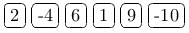
\includegraphics[scale=0.6]{./img/ej1_explicacion1.png}
\caption{Caso ejemplo}
\end{center}
\end{figure}

En este caso, un jugador podr\'ia robar las cartas 2, -4 y 6 o -10, 9, 1, 6, pero no 2, 6, 9 ya que no son adyacentes. \\

Para este caso en particular el juego se desarrollar\'ia de la siguiente manera:

\begin{itemize}
\item Mingo toma 5 cartas desde la izquierda (2, -4, 6, 1 y 9) sumando 14 puntos.
\item An\'ibal toma la \'unica carta restante, el -10.
\end{itemize}

El juego lo gana Mingo logrando una diferencia de 24 puntos.

\subsection{Resoluci\'on y demostraci\'on}

Para resolver el problema dado de $C$ cartas de longitud $n$, debemos construir una funcion $F$ tal que F(C[0..n-1]) est\'e definida como "La jugada que logre la mejor diferencia con el oponente, sabiendo que el mismo juega de forma \'optima" \\

Pensando de manera mas precisa la funci\'on, podriamos escribirla como: \\

F(C[0..n-1]) = MAX(Tomar una carta desde la izquierda y restarle F(C[1..n-1]), Tomar dos cartas desde la izquierda y restarle F(C[2..n-1]), ..., Tomar todas las cartas, ... , Tomar n-2 cartas desde la derecha y restarte F(C[0..0])) \\

Como podemos ver, habr\'ia que tomar la m\'axima diferencia de puntos obtenidos entre las cartas que uno toma y las que toma el oponente, que tambien juega de manera \'optima. La jugada del rival es evaluar la misma funci\'on para el resto de las cartas que dejamos. \\

Definamos esta funci\'on recursivamente (usamos una funci\'on $h$ para lograr claridad): \\

$
F(P) =
\left\{
	\begin{array}{ll}
		P_{0}  & \mbox{if } |P| = 1 \\
		max( h_{izq} (0, n), ... , h_{izq} (k, n) , ... , \sum\limits_{i=0}^n P_{i} , h_{der} (n-1, n), ... , h_{der} (k, n) , ... )  & \mbox{if } |P| > 1
	\end{array}
\right.
$ \\

Las funciones $h_{izq}$ y $h_{der}$ devuelven la diferencia de una jugada en particular tomando una cantidad de cartas y restandole el puntaje del rival con las cartas restantes: \\

$h_{izq}(fin, n) =  (\sum\limits_{i=0}^{fin} C_{i}) - F(C[fin+1...n-1])$ \\
$h_{der}(inicio, n) =  (\sum\limits_{i=inicio}^{n-1} C_{i}) - F(C[0...inicio-1])$\\

Podemos interpretar la funci\'on F como un arbol con todas las posibilidades y finalmente nos devuelve la mejor diferencia posible. Como podemos ver en el ejemplo esta clase de problemas tiene solapamiento de subsoluciones, por lo cual una versi\'on recursiva a secas no es la manera \'optima de implementar la soluci\'on. 

\begin{figure}[h]
\begin{center}
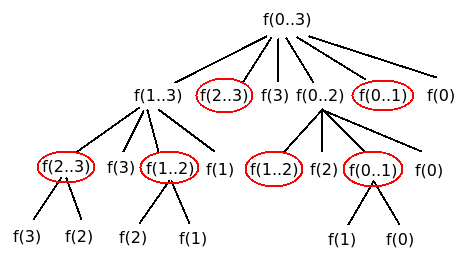
\includegraphics[scale=0.6]{./img/ej1_res1.png}
\caption{\'Arbol representativo de la funci\'on recursiva con los subproblemas requeridos para cada problema en particular, en rojo se marcan los subproblemas solapados}
\end{center}
\end{figure}

Notar que las hojas de este arbol son los casos base y no los consideramos casos repetidos ya que resolverlos tiene una complejidad O(1) como veremos mas adelante. \\

Para evitar volver a calcular subproblemas, decidimos guardar en una matriz de $n*n$ las distintas subsoluciones posibles y en otra tabla de igual tama\~no que combinaci\'on de cartas logr\'o ese resultado. Por ejemplo el subproblema (caso base) F(C[0..0]) est\'a representado por la fila 0 columna 0, pero el resultado al problema total F(C[0..5]) est\'a en la fila 0 columna 5.\\

Sabemos que el caso base de nuestro problema es cuando queda una sola carta. Como estamos obligados a levantar al menos una, es la \'unica opci\'on posible, con lo cual la diagonal de nuestra matriz queda determinada facilmente. 

\begin{figure}[h]
\begin{center}
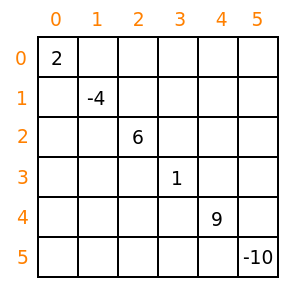
\includegraphics[scale=0.6]{./img/ej1_res2.png}
\caption{Tabla de resultados de F con el problema de ejemplo dado en la secci\'on "Descripci\'on del problema"}
\end{center}
\end{figure}

A partir de ese llenado inicial, podemos ir determinando el resto de los valores de la tabla. En general, un problema de rango $i$ a $j$ siempre usara subproblemas acotados entre estos valores, entonces para un determinado problema F(C[i..j]) alcanza con tener los valores de la tabla de la fila $i$ y de la columna $j$ hasta la posici\'on que estamos calculando.

\newpage

\begin{figure}[h]
\begin{center}
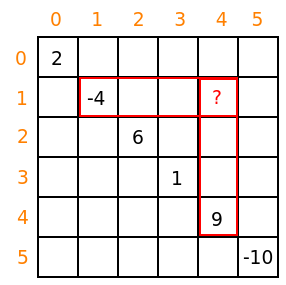
\includegraphics[scale=0.6]{./img/ej1_res3.png}
\caption{Casilleros requeridos para resolver el problema F(C[1..4])}
\end{center}
\end{figure}

Llenando la tabla de abajo hacia arriba y de izquierda a derecha garantiza que siempre tendremos los subproblemas necesarios para llenar el casillero actual. Por ejemplo, para calcular el problema F(C[3..5]) pondriamos en la fila 3 columna 5 el resultado de evaluar MAX(1-F(C[4..5]), 1+9 - F(C[5..5]), 1+9+(-10), -10 - F(C[3..4]), -10+9 - F(C[3..3])), como podemos ver en la tabla todos los subproblemas requeridos ya fueron calculados y sus valores los obtenemos en O(1) en esta ejecuci\'on.

\begin{figure}[h]
\begin{center}
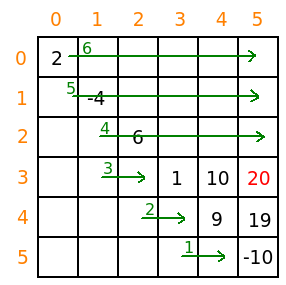
\includegraphics[scale=0.6]{./img/ej1_res4.png}
\caption{Orden de llenado}
\end{center}
\end{figure}

Al terminar de completar la tabla, tendremos el resultado del problema F(C[0..n]) en la fila 0 columna n.

\newpage 

\subsection{Complejidad del algoritmo}

Analizaremos la complejidad del algoritmo propuesto utilizando el siguiente pseudo c\'odigo como gu\'ia: \\

\begin{itemize}
\item crear una tabla de n*n, donde $n$ en es la cantidad de cartas. (Esto demora exactamente $n^2$ iteraciones)
\item para cada fila $f$ (Recorremos las n filas, $n$ iteraciones)
	\begin{itemize}
	\item para cada columna $c$ (Recorremos las n columnas, $n$ iteraciones)
		\begin{itemize}
			\item si es una casilla de la diagonal ($f = c$ caso base) (Esto se realiza en una operaci\'on)
				\begin{itemize}
				\item pongo en $tabla\_resultados(f,c)$ el valor de la carta C[f] (Esto se realiza en una operaci\'on)
				\end{itemize}
			\item si no es diagonal
				\begin{itemize}
				\item guardo en $x$ la suma de todas las cartas (Esto se hace en O(1) usando la tabla de sumas)
				\item guardo en $y$ el maximo valor de todas las combinaciones de tomar cartas desde la izquierda y restarles el puntaje \'optimo del oponente. (Son $n$ iteraciones de posibles subconjuntos de cartas donde se suman en O(1) y se les resta el resultado \'optimo en O(1), ambos datos sacados de la tablas)
				\item guardo en $z$ el maximo valor de todas las combinaciones de tomar cartas desde la derecha y restarles el puntaje \'optimo del oponente. (Son $n$ iteraciones de posibles subconjuntos de cartas donde se suman en O(1) y se les resta el resultado \'optimo en O(1), ambos datos sacados de la tablas)
				\item guardo en $tabla\_resultados(f,c)$ el $max(x,y,z)$ (Asignaci\'on en la tabla, O(1))
				\end{itemize}
		\end{itemize}
	\end{itemize}
\end{itemize}

Para lograr obtener la sumatoria de un rango de cartas en O(1) previamente cargamos una tabla con rangos de sumas de manera similar a la tabla que guarda los resultados de los problemas. Esto se realiza en $n^3$ una \'unica vez antes de comenzar a llenar la tabla de resultados. \\

Finalmente, nuestro algoritmo realiza $O(n^2 * 2*n)$ iteraciones, que es lo mismo que $O(n^2 * 2*n) = O(n^2*n) = O(n^3)$

\newpage

\subsection{C\'odigo fuente}

\lstset{language=C++,
                basicstyle=\ttfamily\footnotesize,
                keywordstyle=\color{blue}\ttfamily,
                stringstyle=\color{red}\ttfamily,
                commentstyle=\color{green}\ttfamily,
                morecomment=[l][\color{magenta}]{\#},
                breaklines=true
}
\begin{lstlisting}

// Lleno todas las posibles subcadenas de sumas en una tabla
for(int i = 0; i<cant_cartas; i++){
	for(int j = 0; j<cant_cartas; j++){
		(*tabla_sumatorias)[i][j] = sumatoria(cartas, i, j); 
	}
}
// Lleno la tabla con los resultados posibles
int cartas_inicio = 0;
int maxval = 0;

for(int i = cant_cartas-1; i>=0; i--){
	
	for(int j = 0; j<cant_cartas; j++){
		
		if(i<=j){
			
			int q = (int) -INFINITY;

			if(i==j){
				// Casos base, la mejor opcion es la unica carta que hay
				cartas_inicio = i;
				q = cartas[j];
				(*tabla_elecciones)[i][j] = pair<int,int>(0,1);
			}else{
				
				// Agarrar todas las cartas
				maxval = max(q, (*tabla_sumatorias)[cartas_inicio][j]);
				// Actualizo la mejor jugada encontrada hasta el momento
				if(maxval>q){
					(*tabla_elecciones)[i][j] = pair<int,int>(0,j-cartas_inicio+1);
				}
				q = maxval;
				
				// Agarrar desde la izquierda y restarle la jugada optima del rival
				for(int k=cartas_inicio; k < j; k++){
					maxval = max(q, (*tabla_sumatorias)[cartas_inicio][k] - (*tabla_resultados)[k+1][j]);
					// Actualizo la mejor jugada encontrada hasta el momento
					if(maxval>q){
						(*tabla_elecciones)[i][j] = pair<int,int>(0,k-cartas_inicio+1);
					}
					q = maxval;
				}
				
				// Agarrar desde la derecha y restarle la jugada optima del rival
				for(int k=j; k > cartas_inicio; k--){
					maxval = max(q, (*tabla_sumatorias)[k][j] - (*tabla_resultados)[cartas_inicio][k-1]);
					// Actualizo la mejor jugada encontrada hasta el momento
					if(maxval>q){
						(*tabla_elecciones)[i][j] = pair<int,int>(1,k-cartas_inicio+1);
					}
					q = maxval;
					
				}

			}
			// q = Max(sumatoria(cartas_{0,0}) - tabla_resultados_{1,n} , ... , sumatoria(cartas_{0,n}))
			(*tabla_resultados)[i][j] = q;
			
		}
		
	}
	
}


\end{lstlisting}

\newpage

\subsection{Casos de prueba}

\subsection{Performance}
